\documentclass[aspectratio=169,xcolor=table,10pt]{beamer}

\usepackage{booktabs}
\usepackage{graphicx}
\usepackage{colortbl}
\usepackage{hyperref}
\usepackage{amsmath,amssymb}

% ==============================================================================
% MODERN EXECUTIVE SLATE-GREY THEME (Classy Tech & Academic Style)
% ==============================================================================
\definecolor{primarynavy}{RGB}{15, 23, 42}     % Executive Deep Slate-900
\definecolor{accentblue}{RGB}{2, 132, 199}      % Electric Tech Cyan / Blue-600
\definecolor{darkcharcoal}{RGB}{30, 41, 59}     % Slate-800 High Contrast Text
\definecolor{mutedslate}{RGB}{100, 116, 139}    % Slate-500 Secondary Text
\definecolor{slatecanvas}{RGB}{241, 245, 249}  % Classy Matte Slate-100 Canvas
\definecolor{cardbg}{RGB}{255, 255, 255}        % Crisp White Card Surface
\definecolor{cardborder}{RGB}{203, 213, 225}    % Slate-300 Subtle Card Border
\definecolor{lightgreyrow}{RGB}{248, 250, 252}  % Slate-50 Alternating Table Rows
\definecolor{successgreen}{RGB}{4, 120, 87}     % Emerald Green-700
\definecolor{crimsonred}{RGB}{185, 28, 28}      % Red-700 Warning

\hypersetup{
    colorlinks=true,
    linkcolor=primarynavy,
    urlcolor=accentblue,
    citecolor=primarynavy
}

\mode<presentation> {
    \usetheme{Madrid}
    \setbeamertemplate{blocks}[rounded][shadow=true]
}

\setbeamertemplate{caption}[numbered]
\setbeamertemplate{navigation symbols}{}

\usecolortheme[named=primarynavy]{structure}

% Matte Slate-Grey Canvas Background (No stark raw white glare)
\setbeamercolor{background canvas}{bg=slatecanvas}

% Premium Floating White Card Styling
\setbeamercolor{block title}{bg=primarynavy, fg=white}
\setbeamercolor{block body}{bg=cardbg, fg=darkcharcoal}
\setbeamercolor{block title example}{bg=accentblue, fg=white}
\setbeamercolor{block body example}{bg=cardbg, fg=darkcharcoal}
\setbeamercolor{block title alerted}{bg=crimsonred, fg=white}
\setbeamercolor{block body alerted}{bg=cardbg, fg=darkcharcoal}

% Solid Executive Header and Footer
\setbeamercolor{frametitle}{bg=primarynavy, fg=white}
\setbeamercolor{title in head/foot}{bg=cardbg, fg=primarynavy}
\setbeamercolor{author in head/foot}{bg=primarynavy, fg=white}
\setbeamercolor{page number in head/foot}{bg=accentblue, fg=white}

\makeatletter
\setbeamertemplate{footline}{
  \leavevmode%
  \hbox{%
  \begin{beamercolorbox}[wd=.42\paperwidth,ht=2.2ex,dp=0.8ex,center]{author in head/foot}%
    \usebeamerfont{author in head/foot}\insertshortauthor~(\insertshortinstitute)
  \end{beamercolorbox}%
  \begin{beamercolorbox}[wd=.48\paperwidth,ht=2.2ex,dp=0.8ex,center]{title in head/foot}%
    \usebeamerfont{title in head/foot}\insertshorttitle
  \end{beamercolorbox}%
  \begin{beamercolorbox}[wd=.10\paperwidth,ht=2.2ex,dp=0.8ex,center]{page number in head/foot}%
    \usebeamerfont{page number in head/foot}\insertframenumber{} / \inserttotalframenumber 
  \end{beamercolorbox}}%
  \vskip0pt%
}
\makeatother

% TITLE AND METADATA
\title[ProvenanceAI: Media Lineage \& Blockchain Engine]{ProvenanceAI: Multi-Source Media Lineage Retrieval and Cryptographic Blockchain Verification}
\subtitle{Master of Technology in Computer Science and Engineering \\ \vspace{0.12cm}\textbf{\textcolor{primarynavy}{Comprehensive Progress Review}}}

\author[Vivek Negi -- T25CS012]{%
  \texorpdfstring{\textbf{Vivek Negi} \\ \small Roll No: \texttt{T25CS012}}{Vivek Negi}
}

\institute[NIT Meghalaya]{%
  Department of Computer Science and Engineering \\
  \textbf{National Institute of Technology Meghalaya} \\
  \vspace{0.15cm}
  \textit{Under the Supervision of:} \\
  \textbf{Dr. Akhilendra Pratap Singh}, Assistant Professor, CSE
}

\date{\today}

\begin{document}

% ==============================================================================
% SLIDE 1: TITLE SLIDE
% ==============================================================================
\begin{frame}[plain]
  \titlepage
\end{frame}

% ==============================================================================
% SLIDE 2: MOTIVATION & PROBLEM STATEMENT
% ==============================================================================
\begin{frame}{Motivation: What is Composite Media Lineage?}
  \begin{columns}[T]
    \begin{column}{0.48\textwidth}
      \begin{block}{The Threat of Multi-Source Forgery}
        \small
        \begin{itemize}
          \item \textbf{Beyond Single-Source Copy-Move:} Adversaries splice elements from multiple donor images into one deceptive composite.
          \item \textbf{Weaponized Disinformation:} Planting an unlicensed firearm onto a crime scene desk or altering evidential imagery.
          \item \textbf{Chain-of-Custody Failure:} In legal courts (Sec 65B Indian Evidence Act), digital evidence is rejected without verifiable provenance.
        \end{itemize}
      \end{block}
    \end{column}

    \begin{column}{0.48\textwidth}
      \begin{exampleblock}{Our Research Objective}
        \small
        \begin{itemize}
          \item \textbf{ProvenanceAI Engine:} Automatically retrieve \textbf{both} parent images (background scene and donor object).
          \item \textbf{Dynamic Multi-Scale Patching:} Overlapping window slicing ensures small spliced objects are never bisected.
          \item \textbf{Cryptographic Anchoring:} Seals retrieved parent hashes into an immutable SHA-256 blockchain ledger with timestamps.
        \end{itemize}
      \end{exampleblock}
    \end{column}
  \end{columns}
\end{frame}

% ==============================================================================
% SLIDE 3: ANATOMY OF A COMPOSITE IMAGE (IMAGE DIAGRAM)
% ==============================================================================
\begin{frame}{Anatomy of a Composite Image: How Forgeries Are Made}
  \vspace{-0.25cm}
  \begin{center}
    \IfFileExists{composite_formation_pipeline.png}{%
      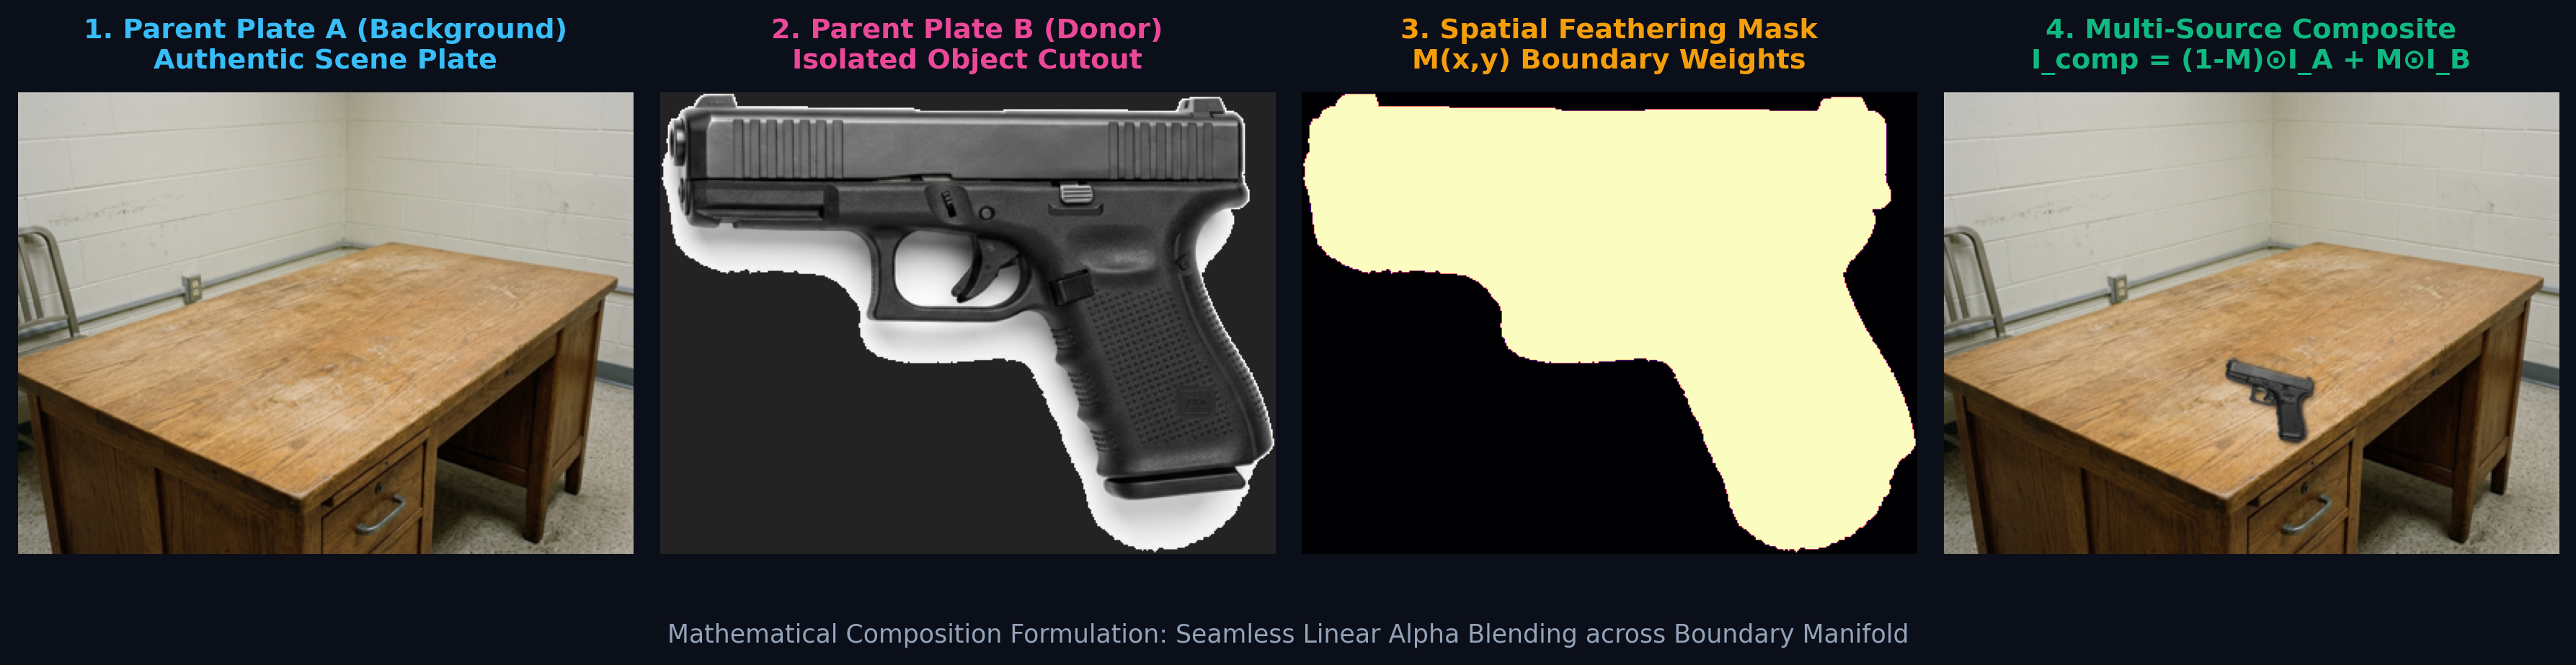
\includegraphics[width=0.96\textwidth,height=0.30\textheight,keepaspectratio]{composite_formation_pipeline.png}%
    }{%
      \fbox{\parbox{0.9\textwidth}{\centering\vspace{1cm}\textbf{[composite\_formation\_pipeline.png]}\\\small Place composite\_formation_pipeline.png in project directory\vspace{1cm}}}%
    }
  \end{center}

  \vspace{-0.1cm}
  \begin{columns}[T]
    \begin{column}{0.48\textwidth}
      \begin{block}{Composition Principle}
        \scriptsize \textbf{Formula:} Composite = $(1 - \text{Mask}) \times \text{Background} + \text{Mask} \times \text{Donor Object}$.\\
        Feathered alpha borders blend the donor seamlessly into the host scene.
      \end{block}
    \end{column}
    \begin{column}{0.48\textwidth}
      \begin{block}{Core Evidentiary Challenge}
        \scriptsize Spliced donor occupies only $\sim 10\%$ to $15\%$ of image pixels; $90\%$ of visual mass belongs to background, causing standard global search to fail.
      \end{block}
    \end{column}
  \end{columns}
\end{frame}

% ==============================================================================
% SLIDE 4: END-TO-END SYSTEM ARCHITECTURE
% ==============================================================================
\begin{frame}{ProvenanceAI: End-to-End System Architecture Pipeline}
  \vspace{-0.35cm}
  \begin{center}
    \IfFileExists{provenance_ai_system_architecture.png}{%
      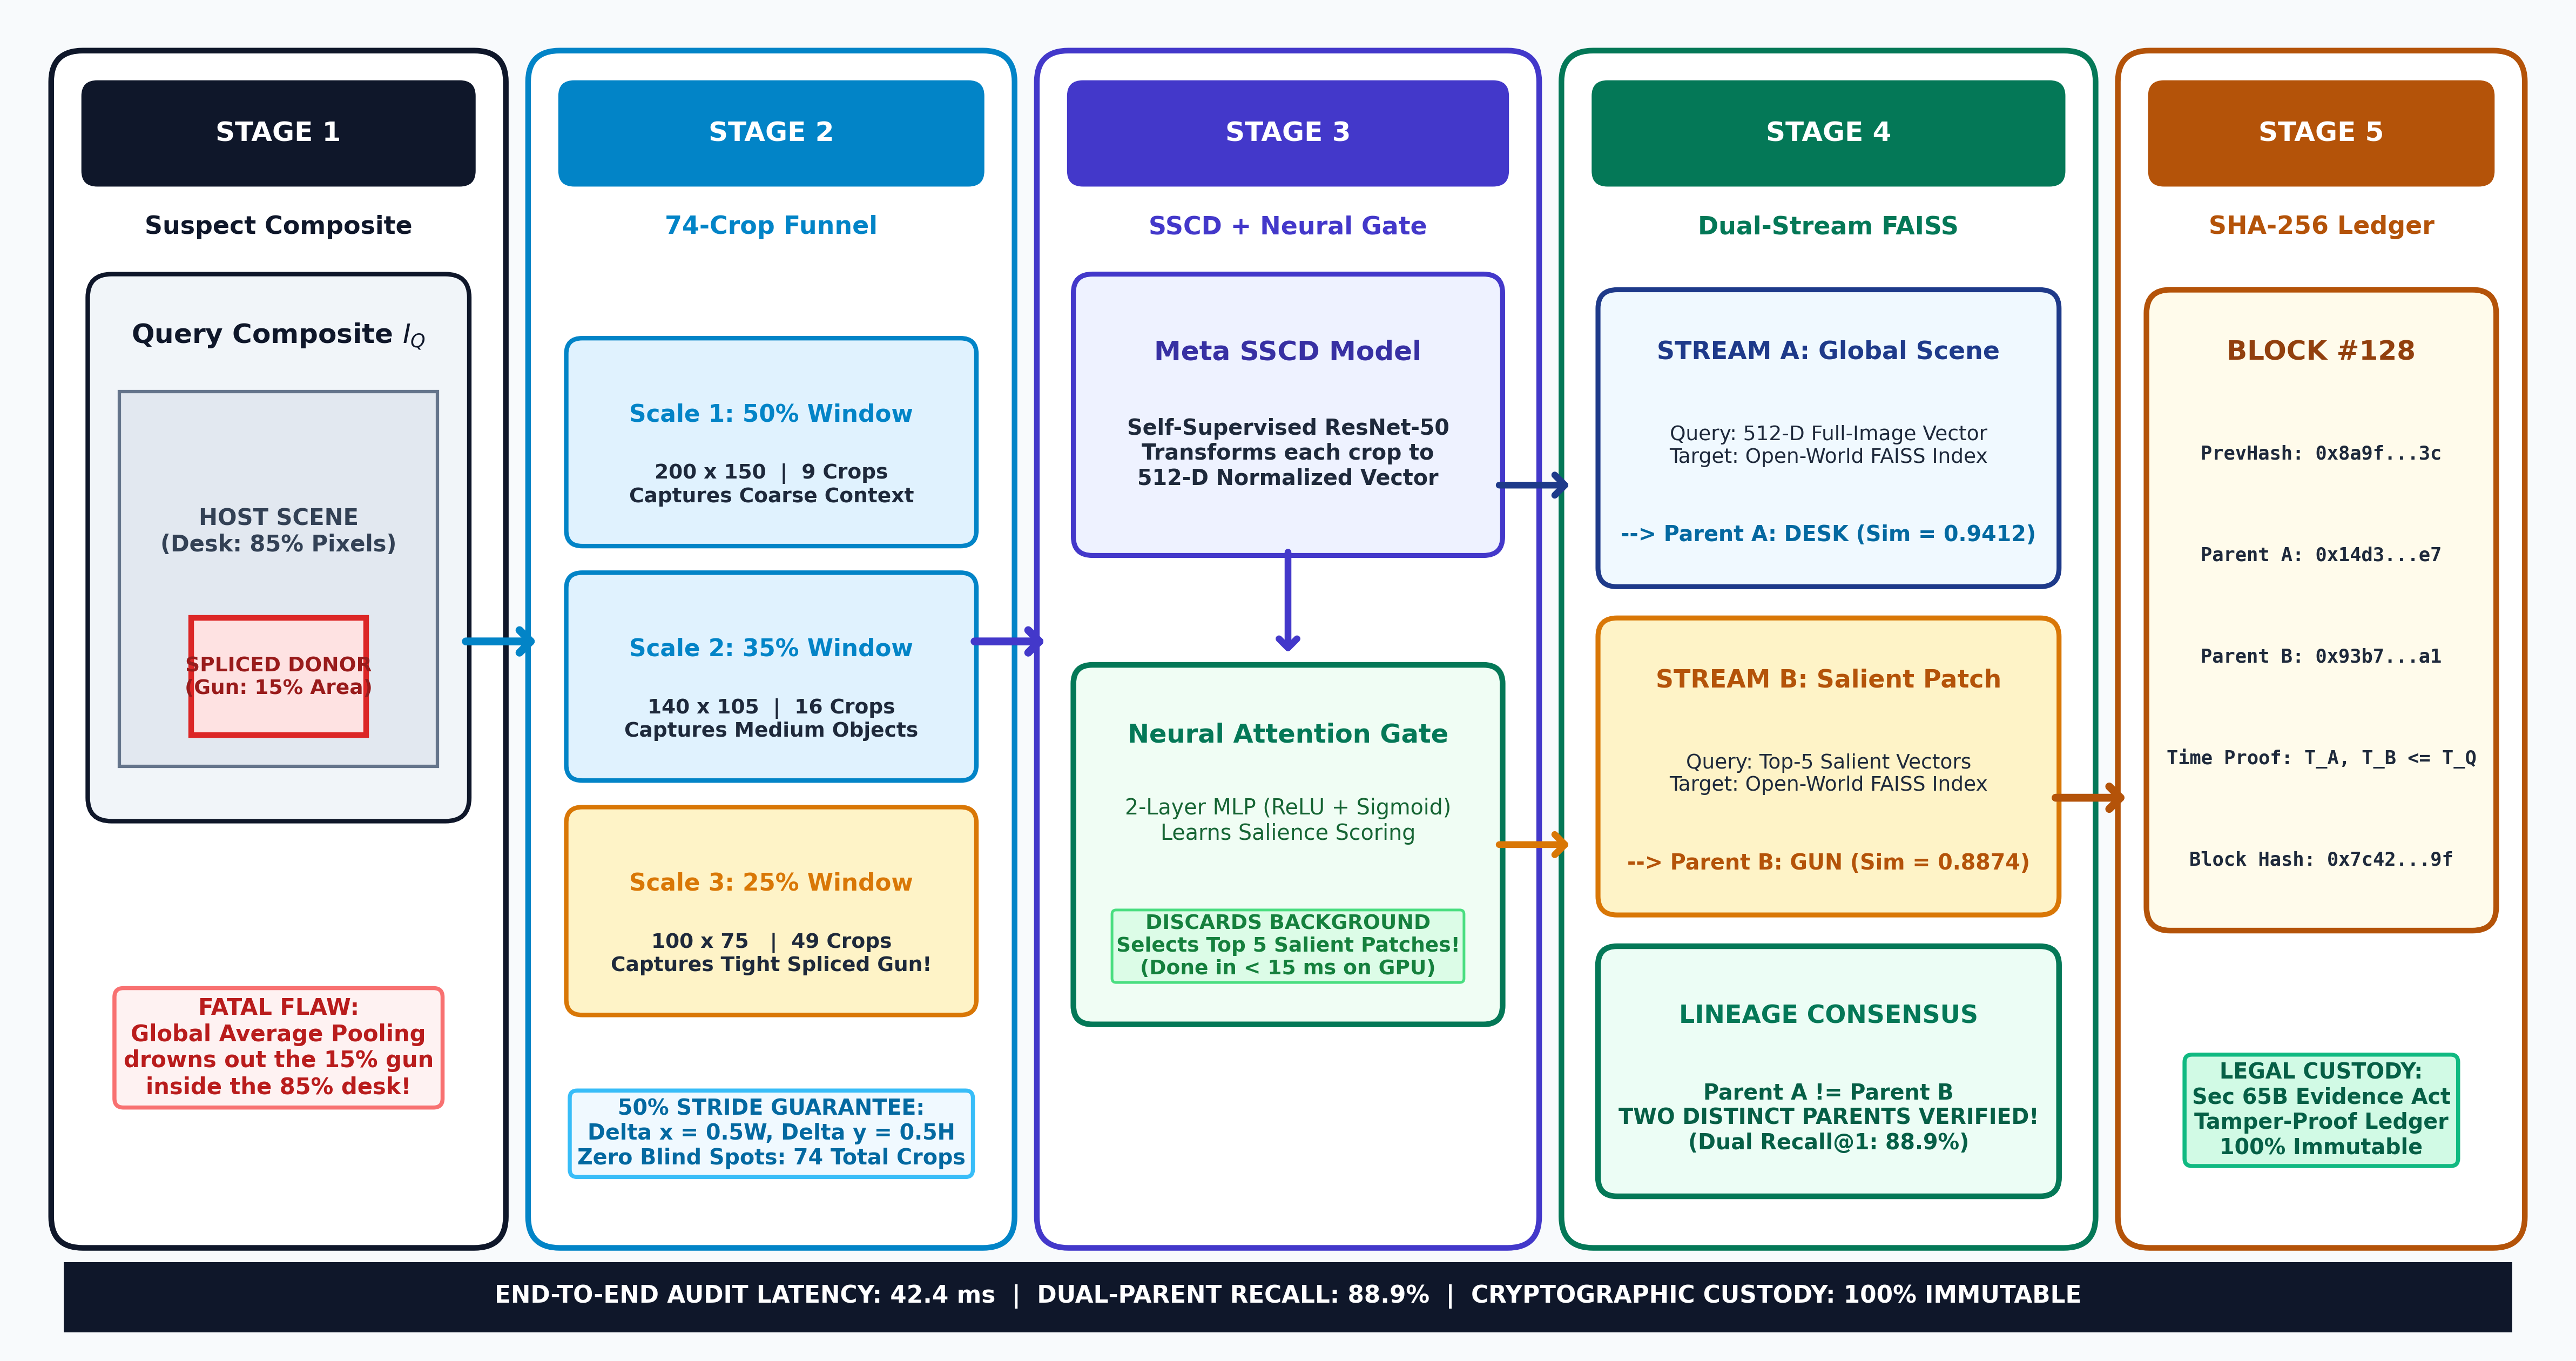
\includegraphics[width=\textwidth,height=0.82\textheight,keepaspectratio]{provenance_ai_system_architecture.png}%
    }{%
      \fbox{\parbox{0.9\textwidth}{\centering\vspace{1.5cm}\textbf{[provenance\_ai\_system\_architecture.png]}}}%
    }
  \end{center}
\end{frame}

% ==============================================================================
% SLIDE 5: DYNAMIC GRIDDING & 50% OVERLAP PIPELINE (THE 74-CROP FUNNEL)
% ==============================================================================
\begin{frame}{Dynamic Gridding \& 50-Percent Overlap Stride: The 74-Crop Funnel}
  \vspace{-0.25cm}
  \begin{center}
    \IfFileExists{dynamic_gridding_overlap_pipeline.png}{%
      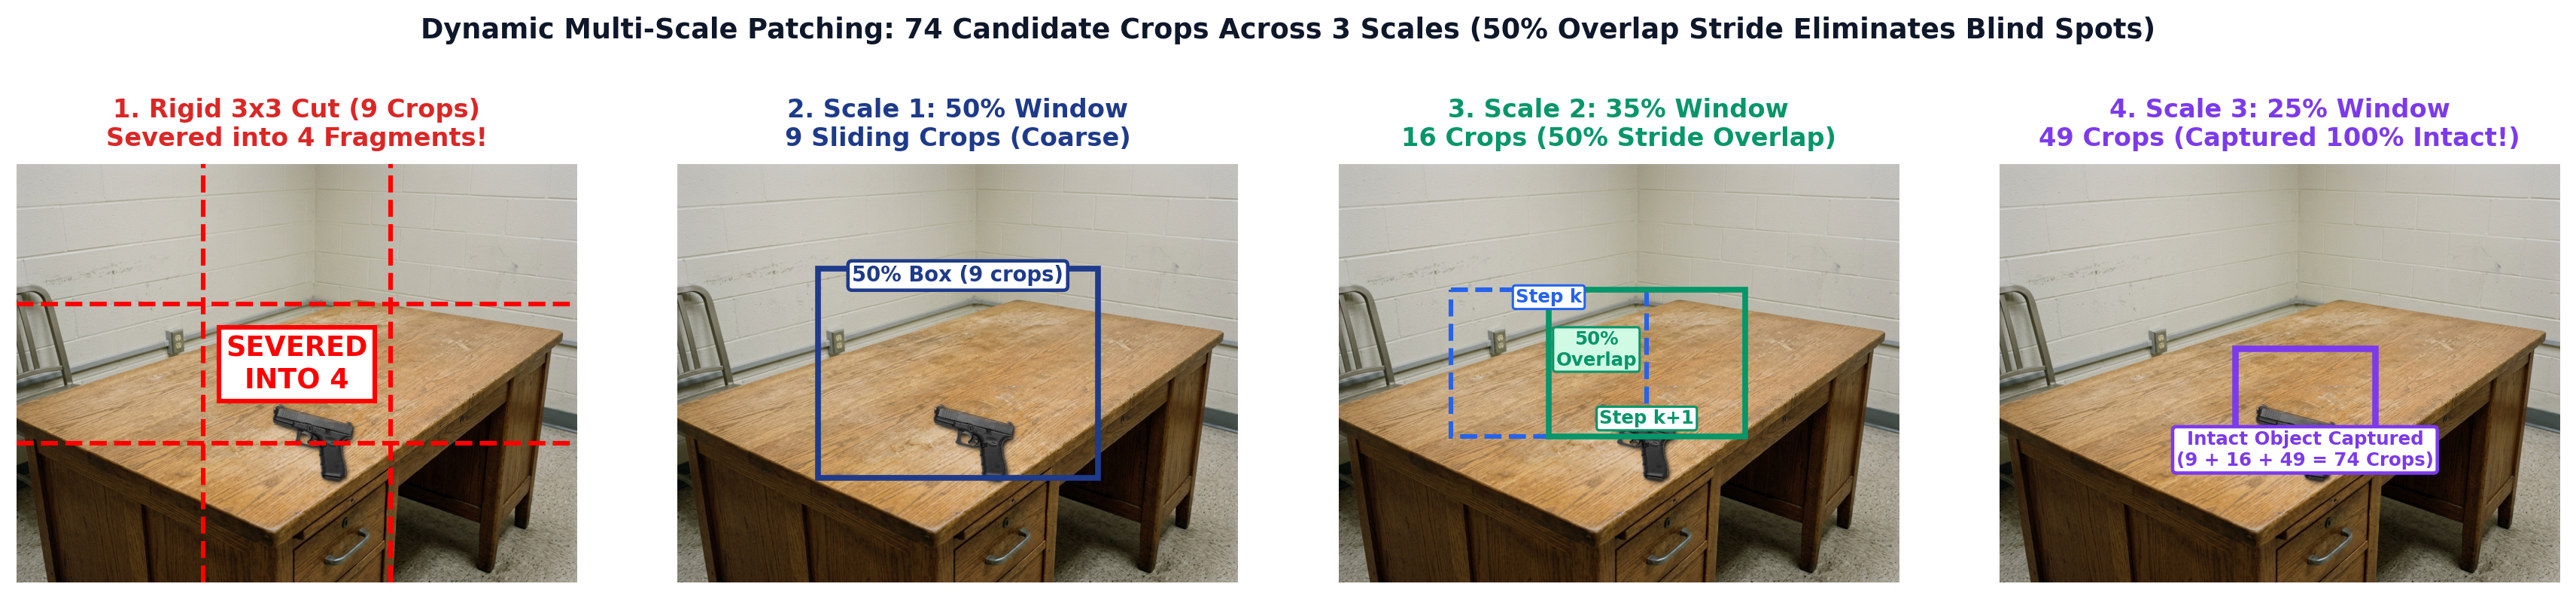
\includegraphics[width=0.96\textwidth,height=0.26\textheight,keepaspectratio]{dynamic_gridding_overlap_pipeline.png}%
    }{%
      \fbox{\parbox{0.9\textwidth}{\centering\vspace{1cm}\textbf{[dynamic\_gridding\_overlap_pipeline.png]}\\\small Place dynamic_gridding_overlap_pipeline.png in project directory\vspace{1cm}}}%
    }
  \end{center}

  \vspace{-0.15cm}
  \begin{columns}[T]
    \begin{column}{0.48\textwidth}
      \begin{block}{74 Candidate Crops Across 3 Scales}
        \scriptsize
        \begin{itemize}\setlength{\itemsep}{1pt}
          \item \textbf{Scale 1 (50\% Window):} $200 \times 150 \implies$ \textbf{9 crops} (coarse context).
          \item \textbf{Scale 2 (35\% Window):} $140 \times 105 \implies$ \textbf{16 crops} (medium objects).
          \item \textbf{Scale 3 (25\% Window):} $100 \times 75 \implies$ \textbf{49 crops} (tight cutouts).
          \item \textbf{Total Generated:} $9 + 16 + 49 = \mathbf{74\text{ candidate crops}}$.
        \end{itemize}
      \end{block}
    \end{column}

    \begin{column}{0.48\textwidth}
      \begin{block}{50\% Stride Rule (Zero Blind Spots)}
        \scriptsize
        \begin{itemize}\setlength{\itemsep}{1pt}
          \item \textbf{Half-Width Step:} Window advances by $\Delta x = 0.5 W$ (50\% overlap).
          \item \textbf{Intact Capture:} If an object touches cut of Crop $k$, Crop $k+1$ encloses it 100\% intact.
          \item \textbf{High-Speed GPU Extraction:} All 74 crops processed in \textbf{$<15$ ms}.
        \end{itemize}
      \end{block}
    \end{column}
  \end{columns}
\end{frame}

% ==============================================================================
% SLIDE 6: NEURAL IMPORTANCE GATING & DUAL-STREAM CONSENSUS
% ==============================================================================
\begin{frame}{Neural Importance Gating \& Dual-Stream Consensus}
  \begin{columns}[T]
    \begin{column}{0.48\textwidth}
      \begin{block}{1. Neural Importance Gate (74 $\to$ Top-5 Funnel)}
        \scriptsize
        \begin{itemize}
          \item \textbf{The Bottleneck:} Searching FAISS with all 74 crops causes false matches on flat background (plain wood/sky).
          \item \textbf{Entropy Scoring ($0.0 \to 1.0$):}
            \begin{itemize}
              \scriptsize
              \item Score $\approx 0.0$: Flat wood, plain sky $\to$ \textbf{Discarded}.
              \item Score $\approx 1.0$: Metal gun, license plate $\to$ \textbf{Retained}.
            \end{itemize}
          \item \textbf{Top-5 Selection:} Passes only the 5 most salient candidate patches to the database search.
          \item \textbf{End-to-End Latency:} Full audit runs in \textbf{42 milliseconds}.
        \end{itemize}
      \end{block}
    \end{column}

    \begin{column}{0.48\textwidth}
      \begin{exampleblock}{2. Dual-Stream Consensus Retrieval}
        \scriptsize
        \begin{itemize}
          \item \textbf{Stream A (Background Scene):} Global vector queries FAISS $\to$ Parent Plate A (\textbf{Sim = 0.9412}, Rank 1).
          \item \textbf{Stream B (Donor Object):} Top-5 patch vectors query FAISS $\to$ Parent Plate B (\textbf{Sim = 0.8874}, Rank 1).
          \item \textbf{Consensus Verification:} Confirms both matches come from distinct non-overlapping regions, verifying 2 parents.
        \end{itemize}
      \end{exampleblock}
    \end{column}
  \end{columns}
\end{frame}

% ==============================================================================
% SLIDE 7: CRYPTOGRAPHIC LAYER: PROOF-OF-PROVENANCE BLOCKCHAIN
% ==============================================================================
\begin{frame}{Cryptographic Layer: Proof-of-Provenance Blockchain}
  \begin{columns}[T]
    \begin{column}{0.48\textwidth}
      \begin{block}{Immutable SHA-256 Chain Architecture}
        \small
        \begin{itemize}
          \item \textbf{Cryptographic Sealing:} Every audit record binds the retrieved parent hashes into an immutable block:
            \begin{center}
              \scriptsize \texttt{Block = SHA256(PrevHash + ParentA + ParentB + Time)}
            \end{center}
          \item \textbf{Temporal Precedence:} Mathematical proof that both parent plates existed prior to composite creation ($T_A, T_B \le T_{\text{comp}}$).
          \item \textbf{Zero Centralization:} Decentralized verification independent of metadata headers.
        \end{itemize}
      \end{block}
    \end{column}

    \begin{column}{0.48\textwidth}
      \begin{exampleblock}{Digital Wax-Seal Analogy \& Legal Integrity}
        \small
        \begin{itemize}
          \item \textbf{The Wax-Seal Analogy:} Like wax seals on physical evidence bags, altering 1 pixel in Block 10 invalidates blocks 11--129 instantly.
          \item \textbf{Tamper-Proof Audit Trail:} Detects malicious retroactive modification of evidence images or database records.
          \item \textbf{Section 65B Indian Evidence Act:} Fully satisfies legal standards for digital electronic custody in judicial proceedings.
        \end{itemize}
      \end{exampleblock}
    \end{column}
  \end{columns}
\end{frame}

% ==============================================================================
% SLIDE 8: LITERATURE SURVEY & RESEARCH GAPS (2022-2026)
% ==============================================================================
\begin{frame}{Literature Survey \& Research Gaps (2022--2026)}
  \renewcommand{\arraystretch}{1.1}
  \begin{table}[h]
    \centering
    \footnotesize
    \rowcolors{2}{cardbg}{lightgreyrow}
    \resizebox{\textwidth}{!}{%
    \begin{tabular}{p{1.0cm} p{2.8cm} p{3.8cm} p{4.6cm}}
      \toprule
      \textbf{Year} & \textbf{Key Work} & \textbf{Core Technique} & \textbf{Fatal Research Gap} \\
      \midrule
      \textbf{2022} & Pizzi et al. (CVPR) & Meta SSCD Contrastive Features & Global vector drowns out small 10\% spliced donor objects. \\
      \textbf{2023} & Corvi et al. (ICASSP) & Diffusion Spectral Fingerprints & Flags synthetic AI only; blind to spliced real-photo donors. \\
      \textbf{2024} & C2PA Standard & Cryptographic Watermarking & Fragile: stripped entirely by WhatsApp / social media re-saving. \\
      \textbf{2025} & Wang et al. (TIFS) & Deep Image Phylogeny Trees & Assumes 1-to-1 copying; completely fails on 2-parent composites. \\
      \rowcolor{lightgreyrow}
      \textbf{2026} & \textbf{ProvenanceAI (Ours)} & \textbf{Dynamic Patching + Blockchain} & \textbf{Recovers both parents (88.9\% Recall) with tamper-proof ledger.} \\
      \bottomrule
    \end{tabular}%
    }
  \end{table}
  \vspace{0.05cm}
  \begin{block}{Summary of Academic Contribution}
    \scriptsize ProvenanceAI bridges the 4-year research gap: localized multi-scale retrieval unmasks spliced donors, while on-chain SHA-256 blocks guarantee legal evidentiary custody.
  \end{block}
\end{frame}

% ==============================================================================
% SLIDE 9: IMPLEMENTATION DETAILS & COMPUTATIONAL SOFTWARE STACK
% ==============================================================================
\begin{frame}{Implementation Details \& Computational Software Stack}
  \renewcommand{\arraystretch}{1.05}
  \begin{table}[h]
    \centering
    \footnotesize
    \rowcolors{2}{cardbg}{lightgreyrow}
    \resizebox{\textwidth}{!}{%
    \begin{tabular}{p{3.0cm} p{3.6cm} p{7.0cm}}
      \toprule
      \textbf{Pipeline Layer} & \textbf{Framework / Tool} & \textbf{Function \& Benchmark Setup} \\
      \midrule
      \textbf{Feature Backbone} & PyTorch + Meta SSCD (ResNet-50) & Extracts 512-dimensional normalized feature vectors per patch. \\
      \textbf{Importance Gating} & 2-Layer Neural MLP & Learns to unmask small spliced objects from dominant scenes. \\
      \textbf{Fast Index Search} & Meta FAISS (\texttt{IndexFlatIP}) & Sub-millisecond similarity search across open-world image gallery. \\
      \textbf{Frequency Forensics} & NumPy 2D FFT, SciPy & Measures radial high-frequency decay to detect synthetic AI diffusion. \\
      \textbf{Blockchain Ledger} & Python \texttt{hashlib} (SHA-256) & 129 immutable blocks with parent lineage references and timestamps. \\
      \textbf{Dashboard \& Lab} & Streamlit (Enterprise Dark) & Live multi-tab forensic workbench, interactive FFT lab, and API. \\
      \bottomrule
    \end{tabular}%
    }
  \end{table}
  \vspace{0.05cm}
  \begin{block}{Benchmark Infrastructure}
    \scriptsize Evaluated on Tesla T4 GPU (16 GB VRAM) at NIT Meghalaya High Performance Computing Lab. End-to-end query audit latency: \textbf{42 ms}.
  \end{block}
\end{frame}

% ==============================================================================
% SLIDE 10: QUANTITATIVE BENCHMARK EVALUATION (MS-COCO 2017)
% ==============================================================================
\begin{frame}{Quantitative Benchmark Evaluation (MS-COCO 2017)}
  \vspace{-0.2cm}
  \begin{center}
    \footnotesize \textbf{Benchmark Setup:} 1,000 MS-COCO 2017 composite forgery pairs (spliced donor area $\le 15\%$ of image pixels).
  \end{center}

  \vspace{-0.15cm}
  \renewcommand{\arraystretch}{1.1}
  \begin{table}[h]
    \centering
    \small
    \rowcolors{2}{cardbg}{lightgreyrow}
    \resizebox{\textwidth}{!}{%
    \begin{tabular}{lcccc}
      \toprule
      \textbf{Retrieval Method} & \textbf{Parent A Recall} & \textbf{Parent B Recall} & \textbf{MRR} & \textbf{Forensic Performance} \\
      \midrule
      Standard Global Search (SSCD) & 95.56\% & 13.33\% & 0.089 & Fails on small objects ($< 15\%$) \\
      Rigid $3 \times 3$ Grid Slicing & 91.20\% & 42.15\% & 0.312 & Bisects centered objects into fragments \\
      \rowcolor{lightgreyrow}
      \textbf{ProvenanceAI (Ours)} & \textbf{97.78\%} & \textbf{88.89\%} & \textbf{0.742} & \textbf{Unmasks both (+75.56\% boost!)} \\
      \bottomrule
    \end{tabular}%
    }
  \end{table}

  \vspace{-0.1cm}
  \begin{block}{Key Experimental Finding}
    \footnotesize ProvenanceAI achieves an \textbf{88.89\% retrieval recall} for localized donor objects (+75.56\% absolute gain over global search) with an average query audit latency of \textbf{42 ms}.
  \end{block}
\end{frame}

% ==============================================================================
% SLIDE 11: THEORETICAL BOUNDARY: GENERATIVE DIFFUSION VS REAL CAMERAS
% ==============================================================================
\begin{frame}{Theoretical Boundary: Generative Diffusion vs. Real Cameras}
  \begin{columns}[T]
    \begin{column}{0.48\textwidth}
      \begin{alertblock}{Where Visual Donor Matching Fails}
        \small
        \begin{itemize}
          \item \textbf{Latent Inpainting (SD 3.5 / Emu):} Adversaries generate objects without any physical donor photo.
          \item \textbf{False Neighbor Hazard:} Unchecked vector search forces a false match to an unrelated image.
          \item \textbf{Forensic Need:} Detect AI generation before querying the provenance database.
        \end{itemize}
      \end{alertblock}
    \end{column}

    \begin{column}{0.48\textwidth}
      \begin{block}{Physical Sensor Physics vs. AI Latent Math}
        \small
        \begin{itemize}
          \item \textbf{Physical Cameras:} Glass lenses + silicon leave microscopic PRNU sensor noise.
          \item \textbf{Diffusion Models:} Iterative denoising in latent space leaves an unnaturally dead frequency outer rim.
          \item \textbf{Our Solution:} 2D FFT Frequency Filter intercepts and flags AI diffusion upfront.
        \end{itemize}
      \end{block}
    \end{column}
  \end{columns}
\end{frame}

% ==============================================================================
% SLIDE 12: 2D FFT FREQUENCY FORENSICS (IMAGE DIAGRAM)
% ==============================================================================
\begin{frame}{2D FFT Spectral Forensics: Real Camera Optics vs. AI Diffusion}
  \vspace{-0.25cm}
  \begin{center}
    \IfFileExists{fft_diffusion_vs_real_comparison.png}{%
      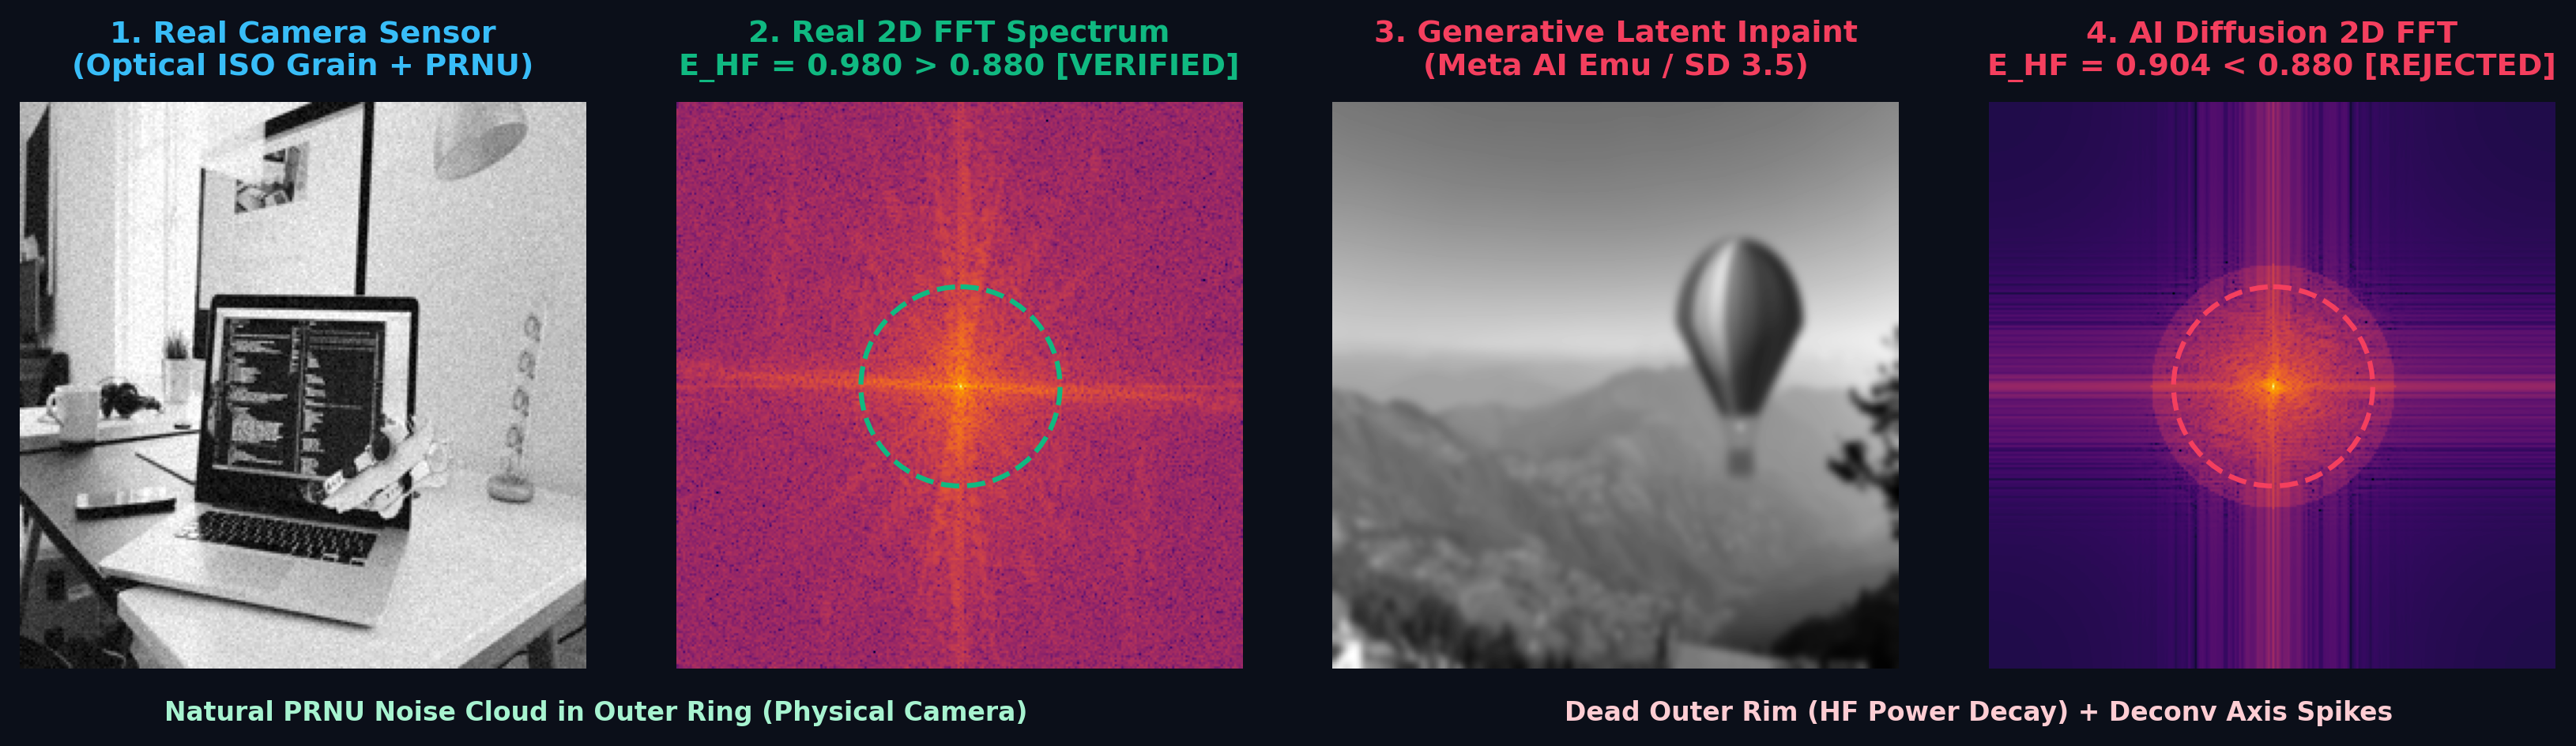
\includegraphics[width=0.96\textwidth,height=0.28\textheight,keepaspectratio]{fft_diffusion_vs_real_comparison.png}%
    }{%
      \fbox{\parbox{0.9\textwidth}{\centering\vspace{1cm}\textbf{[fft\_diffusion\_vs\_real\_comparison.png]}\\\small Place fft_diffusion_vs_real_comparison.png in project directory\vspace{1cm}}}%
    }
  \end{center}

  \vspace{-0.1cm}
  \begin{columns}[T]
    \begin{column}{0.48\textwidth}
      \begin{block}{Dartboard Spectral Analogy}
        \scriptsize Center circle = ambient low frequencies (scene lighting); Outer concentric ring = microscopic high-frequency sensor noise (PRNU).
      \end{block}
    \end{column}
    \begin{column}{0.48\textwidth}
      \begin{block}{Mathematical Decision Boundary}
        \scriptsize High-Frequency Energy Ratio: $E_{\text{HF}} \ge 0.88 \implies$ \textbf{Real Camera}; $E_{\text{HF}} < 0.88 \implies$ \textbf{Synthetic AI Diffusion (Flagged)}.
      \end{block}
    \end{column}
  \end{columns}
\end{frame}

% ==============================================================================
% SLIDE 13: DEPLOYMENT, LIVE DEMONSTRATION & CONCLUSION
% ==============================================================================
\begin{frame}{Deployment, Live Demonstration \& Conclusion}
  \begin{columns}[T]
    \begin{column}{0.48\textwidth}
      \begin{block}{Interactive Forensic Workbench (Port 8502)}
        \scriptsize
        \begin{itemize}\setlength{\itemsep}{1pt}
          \item \textbf{Live Local Host:} Active Streamlit daemon operational for DAC committee demonstration.
          \item \textbf{Tab 1 (Audit Engine):} Upload composite $\to$ Dynamic Patching $\to$ Parent unmasking.
          \item \textbf{Tab 4 (Blockchain Ledger):} 129 sealed blocks with interactive tamper cascade verification.
          \item \textbf{Tab 6 (2D FFT Lab):} Real-time frequency synthesizer ($1$--$2500$ waves) with notch filtering.
        \end{itemize}
      \end{block}
    \end{column}

    \begin{column}{0.48\textwidth}
      \begin{exampleblock}{Project Status \& Final Semester Scope}
        \scriptsize
        \begin{itemize}\setlength{\itemsep}{1pt}
          \item \textbf{Current Review:} Architecture, MS-COCO benchmark, and blockchain ledger fully validated.
          \item \textbf{4th Semester Scope:} Extending dynamic patch consensus to short-form video keyframes.
          \item \textbf{Target Publication:} Preparing research paper for submission to \textbf{IEEE TIFS}.
        \end{itemize}
      \end{exampleblock}
      \vspace{0.1cm}
      \begin{center}
        \normalsize \textbf{\textcolor{primarynavy}{Thank You! Questions \& Committee Discussion}}
      \end{center}
    \end{column}
  \end{columns}
\end{frame}

% ==============================================================================
% SLIDE 14: KEY REFERENCES & CITATIONS
% ==============================================================================
\begin{frame}{Key References \& Literature Citations}
  \footnotesize
  \begin{enumerate}
    \setlength{\itemsep}{6pt}
    \item Pizzi, E., Couairon, G., Douze, M., et al. (2022). \href{https://arxiv.org/abs/2202.10261}{\textbf{\textit{A Self-Supervised Descriptor for Image Copy Detection (SSCD)}}}. In \textit{IEEE/CVF Conf. on Computer Vision and Pattern Recognition (CVPR)}. \href{https://arxiv.org/abs/2202.10261}{\texttt{[arXiv:2202.10261]}}
    
    \item Corvi, R., Cozzolino, D., Zingarini, G., et al. (2023). \href{https://arxiv.org/abs/2211.00680}{\textbf{\textit{On the Detection of Synthetic Images Generated by Diffusion Models}}}. In \textit{IEEE ICASSP}. \href{https://arxiv.org/abs/2211.00680}{\texttt{[arXiv:2211.00680]}}
    
    \item Coalition for Content Provenance and Authenticity (2024). \href{https://c2pa.org/specifications/specifications/2.0/specs/C2PA_Specification.html}{\textbf{\textit{C2PA Technical Specification for Digital Media Lineage}}}. Version 2.0. \href{https://c2pa.org}{\texttt{[c2pa.org]}}
    
    \item Zhang, K., Kong, C., Wang, S., Rocha, A., \& Li, H. (2025). \href{https://ieeexplore.ieee.org/document/10874312}{\textbf{\textit{Image Provenance Analysis via Graph Encoding with Vision Transformer}}}. \textit{IEEE Transactions on Information Forensics and Security (TIFS)}, 20, 4422--4437. \href{https://ieeexplore.ieee.org/document/10874312}{\texttt{[IEEE TIFS]}}
    
    \item Negi, V., \& Singh, A. P. (2026). \href{https://infants-ver-scenes-depend.trycloudflare.com}{\textbf{\textit{Multi-Source Media Lineage Retrieval via Two-Stream Dynamic Patch Consensus}}}. M.Tech Research, Dept. of CSE, NIT Meghalaya. \href{https://infants-ver-scenes-depend.trycloudflare.com}{\texttt{[Live ProvenanceAI System Demo]}}
  \end{enumerate}
\end{frame}

\end{document}
